\newpage

\begin{figure}[h]
\centering
{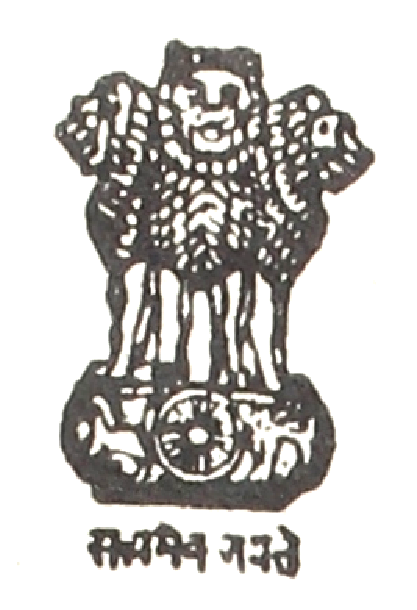
\includegraphics[scale=.25]{0345.eps}}
\end{figure}

\begin{center}
{\large\bfseries{\sktf Ba;a:=+ti6a;a;ya;m,a A;Y3a;Da;Za;a;sa;na;m,a}}\\[10pt]
{\Large\bfseries{\sktf .sa;m1\ZM{cLe}.s1k\ZH{-12}{\ZV{4}{x}}+:ta;a;ya;ea;gaH%
\ZS{4}}}\\[30pt]
{\Huge\bfseries{\sktf :pra:(\ZM{pFngFi}a;a;va;l\ZH{-8}{i9}+.a}}
\end{center}


\vskip 3cm

{\rm 
\begin{center}
{\large\bfseries{SANSKRIT COMMISSION}}\\[30pt]
{\large\bfseries{QUESTIONNAIRE}}
\end{center}
}

\vfill

\begin{center}
{\Large\bfseries{\sktf .sa;m1\ZM{cLe}.s1k\ZH{-12}{\ZV{4}{x}}+:ta;a;ya;ea;ga%
\ZF{-}.sa;Y4a;.ca;va;a;l+.yaH\ZS{4}}}\\
{\Large\bfseries{\sktf :pUa;na;a {\sktf 4}}}\\
{\large\bfseries{\sktf k+:a;Y5a:t1Ra;k\ZF{-}:pa;Ea;NRa;ma;a;si6a;a\ZF{,}
.sMa;va;t,a {\sktf 2013}\ZF{,} Za;k+:a;b.d;aH\ZS{4} {\sktf 1878}}}
\end{center}

\newpage

\begin{spacing}{1.15}
{{\sktf \ZS{12}@A\ZS{6}@A ?\ZS{12}@A\ZS{6}@A ;Y2a;va;Y2a;d;tMa Ka;l\ZH{-6}{u}
Ba;va;ta;Ma ya;t,a Ba;a:=+ta;ga;ta;s1ya .sMa;s1k\ZH{-12}{%
\ZV{4}{x}}+:ta;a;Dya;ya;na;s1ya .sa;a;m1\ZM{cLe}.pra;Y3a;ta;k\ZH{-12}{Y2}+:Ma
.sa;ma;va;s1Ta;Ma .sa;vRa;ta;ea;Y2a;d;ZMa :pa;i8a:=+Zi6a;a;l+.Y4a;ya;tMua 1956
;Y2a;k\ZM{l0R}+:s1ta;a;b.d;s1ya A;k2+:ea;ba:=\ZF{-}ma;a;sea
Ba;a:=+ti6a;a;yea;na A;Y3a;Da;Za;a;sa;nea;na} `{\sktf
.sMa;s1k\ZH{-12}{\ZV{4}{x}}+:ta;a;ya;ea;gaH\ZS{4}}'}

\vskip .1cm

{\sktf O;;SaH\ZS{4} A;a;ya;ea;gaH\ZS{4} .s1vi6a;a;ya;Y2a;va;Y2a;va;Da;k+:a;yeR%
a;Sua ;Y2a;va:(\ZM{dGu};a;Y2a;va;d\ZM{fByF0E};a;a;l+.ya;ga;tMa
ta;Y2a;d;ta:=+sMa;s1Ta;a;ga;tMa ..ca .sMa;s1k\ZH{-12}{%
\ZV{4}{x}}+:ta;Y5a;Za;[a;a;Y2a;va;Sa;ya;k\ZH{-12}{M} .sa;Ma;pra;Y3a;ta;k+:m,a
A;a;nua;k\ZH{-12}{U}+:l1yMa ;Y2a;va;l+.ea;k+:Y4a;ya;Sya;Y3a;ta\ZF{,}
o+.pa;k+:l1pa;Y4a;ya;Sya;Y3a;ta ..ca ta;Ma;s1ta;a;n,a
o+.pa;a;ya;Y2a;va;Zea;Sa;a;n,a .sMa;s1k\ZH{-12}{\ZV{4}{x}}+:ta;a;Dya;ya;na;s1y%
a .sMa;s1k\ZH{-12}{\ZV{4}{x}}+:ta\ZF{-}.sMa;Za;ea;Da;na;s1ya ..ca\break A;Y6a;Ba;v\ZV{4}{x}a:;d\ZM{t0Dj0b};yea
\ZS{12}@A}

\vskip .1cm

{\sktf :pa:=+m1\ZM{cLe}.pa:=+a;ga;ta;Ma .sMa;s1k\ZH{-12}{%
\ZV{4}{x}}+:ta;Y5a;Za;[a;a;pra;Na;a;l\ZH{-8}{i9}+.Ma :pa:=\ZH{-6}{i7}+a;[ya
ta:t3a;tya;aH\ZS{4} :k\ZH{-12}{e} :k\ZH{-12}{e} ;Y2a;va;Zea;Sa;aH\ZS{4}
na;vi6a;a;na;Y5a;Za;[a;a;pra;Na;a;l1ya;a;m,a A;nta;Ba;Ra;v.ya;ma;a;na;aH\ZS{4}
o+.pa;yua:j1yea:=+n,a\ZF{,} I+.tyea;ta;d;Y2a;pa A;sa;Ea
;Y2a;va;.ca;a:=+Y4a;ya;Sya;Y3a;ta \ZS{12}@A}

{\sktf ta;m,a O;;nMa ;Y2a;va;Sa;ya;m,a A;Y3a;Da;k\ZH{-12}{\ZV{4}{x}}+:tya
ta;Y2a;d\ZM{oau};d;Ma ma;ta;m,a A;a;va;a;h;Y4a;ya;tua;m,a o+.pa;nya;s1ta;a
I+.yMa :pra;k\ZH{-12}{\ZV{4}{x}}+:tea;na A;a;ya;ea;gea;na
:pra:(\ZM{pFngFi}a;a;va;l\ZH{-8}{i9}+.a \ZS{12}@A I+.yMa ..ca
:pra:(\ZM{pFngFi}a;a;va;l\ZH{-8}{i9}+.a ;Y2a;va;pua;l+.Y2a;va;Sa;ya;a;va;ga;a;%
Y2a;h;ni6a;a \ZS{12}@A .tea;na ;Y2a;h\ZF{,} yea ma;h;a;Ba;a;ga;aH\ZS{4}
o+t1a:=+prea;Sa;Nea;na A;nua;Y6a:ja;G\ZV{4}{x}a;[ea;yuaH\ZS{4}\ZF{,} na
:tEaH\ZS{4} A;va;Zya{;meava} :pra;Y3a;ta;pra:(\ZM{pFngFi}a;m,a o+t1a:=+m,a o+.d;a;h;a;yRa;m,a \ZS{12}@A
ya:t3a ;Y2a;va;Sa;ya;Y2a;va;Zea;Sea yea;Sa;a;m,a A;Y6a;Ba;Y4a;na;vea;ZaH\ZS{4}
.sMa;ba;nDa;Y2a;va;Zea;SaH\ZS{4} va;a ;Y2a;va;Y5a;Za;S1\ZH{-6}{M} :]a;a;nMa
va;a .s1ya;a;t,a\ZF{,} ta:t3a .tea .s1va;ma;tMa ta;d\ZH{-10}{u};pa;ea;d%
\ZM{oaupabj0b};l+.k\ZH{-12}{M} ..ca yua;Y3a;k2+.ja;a;tMa .sa;ma;a;sea;na
:pra;d;ZRa;yea;yuaH\ZS{4}\ZF{,} I+.Y3a;ta .sa;veRa
v.ya;va;h;ta;Ra:=\ZS{1}H\ZS{4} A;m1ya{TyRa};ntea \ZS{12}@A d\ZH{-6}{i6};a;ya;ma;a;na;m,a o+t1a:=\ZH{-6}{M}
:]a;a;pa;k\ZH{-12}{M} va;a yMa :pra:(\ZM{pFngFi}a\ZH{-6}{M}
.s1\ZM{cLe}.p\ZV{4}{x}a;Za;Y3a;ta\ZF{,} ta;s1ya :pra:(\ZM{pFngFi}a;s1ya
A;\ZM{0PqPOM0bvJbPJbEJdE}*:\ZS{2}H\ZS{4} .s1\ZM{cLe}.pa;S1\ZH{-6}{M}
;Y4a;na;d\ZH{-6}{eR};ZyaH\ZS{4} \ZS{12}@A}

\vskip .1cm

{\sktf A;a:\ZM{FPqVOM00gFEILdlXDI}*+:+.Ba;a;Sa;ya;a
.sMa;s1k\ZH{-12}{\ZV{4}{x}}+:ta;Ba;a;Sa;ya;a va;a o+t1a:=+a;Y5a;Na
d;a;ta;v.ya;a;Y4a;na \ZS{12}@A o+t1a:=+a;Y5a;Na ..ca} `{\sktf
.sa;d;s1ya\ZF{-}.sa;Y4a;.ca;vaH\ZS{4}\ZF{,} .sMa;s1k\ZH{-12}{%
\ZV{4}{x}}+:ta;a;ya;ea;gaH\ZS{4}\ZF{,} :pUa;na;a 4}' {\sktf O;;ta;m,a
o+.Y1a;d1+Zya ta;Ta;a :prea;Sa;Ni6a;a;ya;a;Y4a;na\ZF{,} ya;Ta;a 12
;Y2a;q+.sa;m1ba:=\ZF{,} 1956 O;;ta;t,a ;Y2a;d;nMa ya;a;va;t,a
:pra;a;pyea:=+n,a \ZS{12}@A}

\vskip .1cm

{\sktf  I+.d\ZH{-6}{M} ..ca A;pa:=\ZH{-6}{M} v.ya;va;h;ta;Ra:=\ZS{1}H\ZS{4}
:pra;a;TyRa;ntea\ZF{,} ya;t,a .tea .s1vea;Sa;a;m,a o+t1a:=+a;Na;a;m,a
A;va;sa;a;nea ;Y4a;na:jMa .sa;ma;gr4Ma na;a;ma\ZF{,} A;Y3a;Da;k+:a:=+m,a\ZF{,}
A;a;va;a;sa;s1Ta;a;nMa ..ca ;Y4a;l+.Kea;yuaH\ZS{4} \ZS{12}@A\ZS{6}@A}
\end{spacing}
\medskip

{\rm 
You are aware that the Government of India have appointed (in October 1956) a Sanskrit Commission to consider the question of the present state of Sanskrit Education in India.

\vskip .1cm

The commission will, among other things survey the existing facilities for Sanskrit Education in Universities and non-University institutions and make proposals for promoting the study of Sanskrit, including research, It will also examine the traditional system of Sanskrit Education in order to find out what features from it an be usefully incorporated into the modern system.


With a view to eliciting informed public opinion on the subject, the Commission has issued the present Questionnaire. The Questionnaire convers a wide field of inquiry, and it is not intended that all those who are pleased to send replies should necessarily answer every question. Correspondoents are requested to favour the Commission with their views and suggestions on matters in which they are particulary interested or concerrxed, or of, which they have special knowledge. Reasons, in brief, may please be given in support of the views expressed. The number of the question to which the answer or memorandum relates should be clearly indicated.

Replies, in English or Sanskrit, may be kindly sent to `The Member Secretary, Sanskrit Commission, Poona 4', so as to reach him not later than the 12th of December, 1956. 

Correspindents are requested to give their full names, designations, and addresses at the end of their replies.
}

\newpage

\begin{spacing}{1.15}
{\sktf \ZS{12}@A\ZS{6}@A A \ZS{12}@A\ZS{6}@A .sa;a;ma;a;nya;pra;k+.=+Na;m,a
\ZF{-} mUa;l+.BUa;ta;aH\ZS{4} :k\ZH{-12}{e}+:.ca;na
:pra:(\ZM{pFngFi}a;aH\ZS{4} \ZS{12}@A\ZS{6}@A}

\begin{itemize}
  \item[{\sktf 1}.] {\sktf k+:a BUa;Y6a;ma;k+:a k+:a;yRa;Y2a;va;Zea;SaH\ZS{4}
va;a .sMa;s1k\ZH{-12}{\ZV{4}{x}}+:ta;Y2a;va;d;a A;d\ZM{fByF0E};a;ta;nea
Ba;a:=+ta;s1ya .=+a;Y2a;S1\ZH{-10}{r1};ya:ji6a;a;va;nea
;Y4a;na;vRa;tRa;Y4a;ya;ta;v.yaH\ZS{4} \ZF{?}}  
  
  \item[{\sktf 2}.] \begin{itemize} 
    \item[({\sktf k})] {\sktf .sMa;s1k\ZH{-12}{\ZV{4}{x}}+:ta;a;Dya;ya;nMa
:pra;Y3a;ta Ba;va;d\ZH{-6}{i6};a;yea k\ZH{-12}{Y2}+:a;d\ZH{-4}{%
\ZV{2}{x}};Zi6a;a .ja;na;a;na;Ma .sa;a;Da;a:=+Ni6a;a
ma;na;ea;v\ZV{4}{x}a;Y5a:t1aH\ZS{4} \ZF{?}}
                        
    \item[({\sktf Ka})] {\sktf :pa;a;F+.Za;a;l+.a;sua\ZF{,}
ma;h;a;Y2a;va;d\ZM{fByF0E};a;a;l+.yea;Sua\ZF{,} ;Y2a;va:(\ZM{dGu};a;Y2a;va;d%
\ZM{fByF0E};a;a;l+.yea;Sua ..ca :pra;va;tRa;ma;a;na;a;t,a
.sMa;s1k\ZH{-12}{\ZV{4}{x}}+:ta;a;Dya;ya;na;a;t,a v.ya;Y3a;ta;=\ZH{-6}{e}+k%
\ZH{-12}{e}+:Na\ZF{,} ;k\ZH{-12}{E}\ZS{3}H\ZS{4} ;k\ZH{-12}{E}\ZS{3}H\ZS{4}
o+.pa;a;ya;a;nta;=\ZH{-6}{E}\ZS{1}H\ZS{4} Ba;va;d\ZH{-6}{i6};a;yea
:pra;d\ZH{-6}{e};Zea .sMa;s1k\ZH{-12}{\ZV{4}{x}}+:ta;Y2a;va;d%
\ZM{fByF0E};a;a;ya;aH\ZS{4} A;Y6a;Ba;v\ZV{4}{x}a;Y4a:;d\ZM{t0Dj0b}H\ZS{4}
;Y2a;k\ZM{l0R}+:ya;tea\ZF{,} .sMa;s1k\ZH{-12}{\ZV{4}{x}}+:ta;sa;a;Y2a;htyea ta;d;nua;pra;a;Y5a;Na;ta;a;ya;Ma .sMa;s1k\ZH{-12}{\ZV{4}{x}}+:ta;Ea ..ca
A;a;d:=\ZS{1}H\ZS{4} :pa;i8a:=+pa;a;l1ya;tea \ZF{?,}
I\ZH{-6}{R}+.d\ZH{-4}{\ZV{2}{x}};Za;s1ya A;a;d:=+s1ya
A;Y6a;Ba;v\ZV{4}{x}a:;d\ZM{t0Dj0b}\ZH{-6}{e};(\ZM{rac0FI}a A;TeRa
:k\ZH{-12}{e} o+.pa;a;ya;aH\ZS{4} Ba;va;Y5a;;d2\ZM{x0Bi0ed0E}\ZS{1}H\ZS{4}
.sUa;.cya;ntea \ZF{?}}
     \end{itemize}
                       
 \item[{\sktf 3}.] \begin{itemize}
      \item[({\sktf k})] {\sktf ma;a;na;Y2a;va;k\ZH{-12}{Y2}+:a
.sa;Ma;s1k\ZH{-12}{\ZV{4}{x}}+:Y3a;ta;k\ZH{-12}{Y2}+:a ..ca
.sMa;s1k\ZH{-12}{\ZV{4}{x}}+:ta;s1ya A;na;GRa;ta;a;m,a A;a;l+.ea;.cya\ZF{,}
.sMa;s1k\ZH{-12}{\ZV{4}{x}}+:ta;a;Dya;ya;na ;Y2a;va;Sa;yea
ma;h\ZH{-6}{i6};a;yaH\ZS{4} o+;d\ZM{t0Dj0b};ea;Da;na;m,a A;a;d:=\ZH{-6}{M}
..ca Ba;a:=+ti6a;a;ya ga;Na;ta:n:t4a;a;nua;pa;a;Y4a;l+.tea;Sua
na;a;ga;i8a:=+k\ZH{-12}{e}+:Sua .sa;mua;tpa;a;d;Y4a;ya;tMua k+:a;n,a
o+.pa;a;ya;a;n,a o+.pa;a;d\ZH{-6}{e};ya;tvea;na Ba;va;ntaH\ZS{4} .sUa;.ca;yea;yuaH\ZS{4}\ZF{?}}
                      
 \item[({\sktf Ka})] {\sktf k\ZH{-12}{Y2}+:a;d\ZH{-4}{\ZV{2}{x}};%
\ZH{0}{i0//////Y7}a;gBaH\ZS{4} ;Y2a;va;Da;a;Y6a;BaH\ZS{4}} `{\sktf
.sa;a;Y2a;h;tya \ZF{-} A;k+:a;d\ZH{-6}{e};mi6a;a}' {\sktf
\ZF{(}A;\ZH{0}{i0Y7}a;Ka;l\ZF{-}Ba;a:=+ti6a;a;ya\ZF{-}.sa;a;Y2a;h;tya%
\ZF{-}:pa;i8a:=+Sa;t,a\ZF{)} .ja;na;a;na;Ma} {\sktf
.sMa;s1k\ZH{-12}{\ZV{4}{x}}+:ta;va;a:\ZM{0PqPOMDbmQbiX0AXhA}*+;;ya;a;Dya;ya;na%
;s1ya} {\sktf :pra:=+ea;.ca;na;a;ya\ZF{,} ta;Y2a;d\ZM{oau};Sa;yea ..ca
A;a;d:=+sMa;va;DRa;na;a;ya\ZF{,} .sa;a;h;a;yyMa k+:tR2ua Za;\ZM{0NkLNPLPE0DnLDE}*:\ZH{-8}{\ZV{-2}{u}}+:ya;a;t,a \ZF{?}
.tea;Sua .tea;Sua ;Y2a;va;d\ZM{fByF0E};a;a;s1Ta;a;nea;Sua
:pra;Y3a;ta;Y4a;na;Y3a;Da;BUa;ta;a;na;Ma .sMa;s1k\ZH{-12}{%
\ZV{4}{x}}+:ta;gr4a;nTa;a;na;a;m,a \ZF{(}1\ZF{)} A;a:%
\ZM{FPqVOM00gFEILdlXDI}*+:+.Ba;a;Sa;a;ya;Ma \ZF{(}2\ZF{)}
:pra;a;d\ZH{-6}{e};Y5a;Za;k+:Ba;a;Sa;a;sua ..ca A;nua;va;a;d\ZH{-6}{E}H\ZS{4}
.sa;h;k\ZH{-12}{\ZV{4}{x}}+:ta;a;Y4a;na .s1va;l1pa;mUa;l1ya;a;Y4a;na
.sMa;s1k+.=+Na;a;Y4a;na :k\ZH{-12}{e}+:nd\ZP{-8}{-4}{@R}+a;Y3a;Da%
\ZF{-}Za;a;sa;na;s1ya} {\sktf {.=+a:j1ya;a;Y3a;Da}Za;a;sa;na;a;na;Ma} {\sktf ..ca d\ZM{oau};a:=\ZH{-6}{e}+Na}  `{\sktf
.sa;a;Y2a;h;tya\ZF{-}A;k+:a;d\ZH{-6}{e};mi6a;a}' {\sktf .s1va;yMa
:pra;k+:a;Za;yea;t,a A;nyEaH\ZS{4} va;a :pra;k+:a;Zya;ma;a;na;a;Y4a;na
:pua:=+s1k\ZH{-12}{u}+:ya;Ra;t,a\ZF{,} I+.tyea;ta;Y2a;d\ZM{oau};Sa;yea
Ba;va;ta;Ma ;Y2a;k\ZH{-12}{M} ma;ta;m,a\ZF{?}} [{\sktf
ya;va;na\ZF{-}.=+ea;ma;k\ZF{-}Ba;a;Sa;ya;eaH\ZS{4}
;Y4a;l+.\ZH{0}{i0Y7}a;Ka;ta;a;na;Ma gr4a;nTa;a;na;a;m,a
{A;a:\ZM{FPqVOM00gFEILdlXDI}*+:}+.Ba;a:Sa;a;nua;va;a;d\ZF{-}.sa;h;k\ZH{-12}{\ZV{4}{x}}+:ta\ZF{-}.sMa;s1k+.=%
\ZF{-}:Na;a;na;Ma :pra;Na;ya;nea\ZF{,}} `{\sktf l+.ea.O;;ba\ZF{-}{\break}%
\ZM{0NkLNPLPELFI00l}*:+:a;Y6a;sa;k+:l\ZF{-}l+.a;ya;b.ra:=\ZH{-6}{i7}+a}'
{\sktf .sMa;s1Ta;ya;a ya;a .sa:=+a;Ni6a;aH\ZS{4} A;nua;\ZH{0}{i0Y7}a;s1%
\ZM{aLeDDr}:a;ya;tea\ZF{,} .sa;a A:t3a o+.d;a;h;a;ya;Ra \ZS{12}@A}\,]
                      
\item[({\sktf ga})] {\sktf ;Y2a;d\ZM{oau};ti6a;a;ya;s1ya;Ma
:pa;a:\ZM{BNz0dcRfA}*.a;va;Y2a;SRa;ky2+.a;Ma ya;ea:ja;na;a;ya;Ma
.sMa;s1k\ZH{-12}{\ZV{4}{x}}+:ta;Y5a;Za;[a;a;ya;aH\ZS{4}
A;Y6a;Ba;va;DRa;na;a;ya :k\ZH{-12}{e} o+.pa;a;ya;aH\ZS{4}
Ba;va;nm1\ZM{cLe}.a;tea A;va;l+.m1ba;ni6a;a;ya;aH\ZS{4} \ZS{12}@A}
 \end{itemize} 
\end{itemize}
\end{spacing}

{\rm 
\section*{{\rm\bfseries A. General-Some Basic Questions}}

\noindent
\begin{itemize}
  
  \item[1.] What special role has Sanskrit to play in the national life of India to-day?
  
  \item[2.] \begin{itemize}
            \item[(a)] How would you characterize the general sentiment in your part of the conuntry towards the study of Sankrit?  
              
              \item[(b)] Apart from its study in P$\bar{a}$tha$\acute{s}\bar{a}$l$\bar{a}$s, Colleges and Universities, in what other ways are the cultivation of Sanskrit and interest in its literature and culture maintained in your part of the country? What steps would you suggest to promote such interest and cultivation?
             \end{itemize}
  \item[3.]\begin{itemize}
           \item[(a)] In view of the humanistic and cultural value of Sanskrit what steps would you sugeest for engendering among the citizens of the Republic of India a greater awareness for and interest in the study of Sanskrit?
           
           \item[(b)] In what ways can the {\textit {Sahitya Akademi}} help to popularize and promote interest in the study of Sanskrit literature? Should the {\textit {Sahitya Akademi}} in your opinion, undertake and encourage the publication by the Center as well as the States, in cheap editions, of representative Sanskrit texts in the different branches of learning, with accompanying translations in (i) English and (ii) the regional languages (in a style like that of the {\textit {Loeb Classical Library}} of Greek and Latin texts in English, for example)?
           
           \item[(c)] What provisions, in your opinion, need be made in the Second Five Year Plan for the promotion of Sanskrit Education?
           \end{itemize}
\end{itemize}           
}